\subsection{Algoritmo genético}
Para esta práctica se desarrolló un algoritmo genético que se apega al proceso mostrado en la Figura \ref{fig:AG}.

\begin{figure}[htbp]
	\centering
	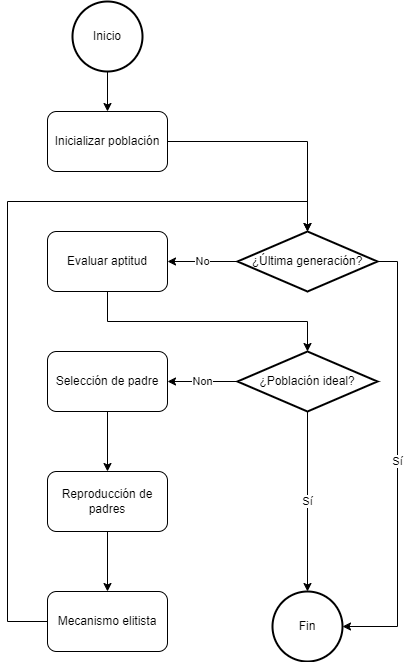
\includegraphics[width=0.45\textwidth]{algoritmo_genetico_proceso}
	\caption{Diagrama de flujo del algoritmo genético implementado.}
	\label{fig:AG}
\end{figure}

Para llevar a cabo dicho proceso, se optó por utilizar el lenguaje de programación Python, donde se diseñaron métodos genéricos para realizar los procesos de generación de población, evaluación de aptitud, selección de individuos, reproducción de individuos, mutación y mecanismos elitistas.


\subsection{Pruebas realizadas}
Se implementó una única combinación de mecanismos, el cuál incluye:

\begin{itemize}
	\item Mecanimo de selección.
	\begin{itemize}
		\item Selección Monogámica Aleatoria (SMA).
		\item Selección Torneo (ST).
	\end{itemize}
	\item Mecanismo de cruza.
	\begin{itemize}
		\item Cruza de un punto (1Px).
		\item Cruza de dos puntos (2Px).
	\end{itemize}
	\item Mutación Scramble (MS).
\end{itemize}

Dichas combinaciones se segmentaron en 3 islas, siguiendo el siguiente patrón:

\begin{itemize}
	\item Isla 1: SMA + 1Px + MS.
	\item Isla 2: ST + 1Px + MS.
	\item Isla 3: ST + 2Px + MS.
\end{itemize}

Este conjunto de islas se entrenó en 3 ocasiones, con el objetivo de generar una vista general del comportamiento de cada algoritmo. En cada caso, el procedimiento se entrenó durante 20 generaciones.

Cabe destacar que, dado que solamente se implementó 1 mecanismo elitista, este fue aplicado a todos los algoritmos por igual. También es importante mencionar que se implementó 1 criterio de paro establecido únicamente por el número de generaciones.

\subsection{Parámetros iniciales}
Se definió la función aptitud como el máximo valor positivo (utilidad) de la suma de los ingresos menos los costos de la producción total de papel. Dicha función de aptitud depende directamente de los siguientes parámetros:

\begin{itemize}
	\item Periodo de producción: 10-50 días.
	\item Cantidad máxima de producción por día: 10-50 toneladas.
	\item Porcentaje mínimo de producción: 10-50 \%.
	\item Producción al día: Cantidad de piezas que se fabrican.
	\item Ganancia al día: Definido como el producto de la producción y el precio.
	\item Costo: Costo del papel a producir según sea su color y grosor.
	\item Precio: Establecida como el doble del costo para garantizar ganancias.
	\item Peso: Peso del papel según su grosor.
\end{itemize}

\subsection{Estimación de precios}
Acorde al color y grosor del papel a producir, se puede consultar la Tabla \ref{tab: precios}.

\begin{table}[htbp]
\centering
\caption{Lista de precios de papel.}
\begin{tabular}{llllllll}
\hline
Color  & Grosor & Costo & Precio & Ganacia & Peso & Producción al día & Gananacia final \\ \hline
Blanco & 1      & 4     & 8      & 4       & 0.1  & 100000            & 400000          \\
Blanco & 2      & 9     & 18     & 9       & 0.2  & 50000             & 450000          \\
Azul   & 1      & 3     & 6      & 3       & 0.1  & 100000            & 300000          \\
Azul   & 2      & 7     & 14     & 7       & 0.2  & 50000             & 350000          \\
Negro  & 1      & 2     & 4      & 2       & 0.1  & 100000            & 200000          \\
Negro  & 2      & 5     & 10     & 5       & 0.2  & 50000             & 250000          \\ \hline
\end{tabular}
\label{tab: precios}
\end{table}

\subsection{Multas}
Cuando se es requerido un cambio en la máquina, existen multas por limpieza establecidas en la Tabla \ref{tab: multas}.

\begin{table}[htbp]
\centering
\caption{Lista de multas por cambio de color.}
\begin{tabular}{llll}
\hline
       & Blanco & Azul  & Negro \\ \hline
Blanco & 0      & 25000 & 25000 \\
Azul   & 25000  & 0     & 25000 \\
Negro  & 50000  & 4     & 0    
\end{tabular}
\label{tab: multas}
\end{table}